% allgem. Dokumentenformat
\documentclass[a4paper,12pt,headsepline,twocolumn]{scrartcl}

% weitere Pakete
% Grafiken aus PNG Dateien einbinden
\usepackage{graphicx}

%deletes first blank page
\usepackage{atbegshi}% http://ctan.org/pkg/atbegshi
\AtBeginDocument{\AtBeginShipoutNext{\AtBeginShipoutDiscard}}

%for links 
\usepackage{color}
\usepackage{hyperref}
\hypersetup{
    colorlinks=true,
    linkcolor=blue,
    urlcolor=red,
    linktoc=all
}
\usepackage{xr}
\externaldocument{Julian.tex}

% Deutsche Sonderzeichen benutzen 
%\usepackage{ngerman}

% deutsche Silbentrennung
\usepackage[ngerman]{babel}

% Eurozeichen einbinden
\usepackage[right]{eurosym}

% Umlaute unter UTF8 nutzen
\usepackage[utf8]{inputenc}

% Zeichenencoding
\usepackage[T1]{fontenc}

\usepackage{lmodern}
\usepackage{fix-cm}

% floatende Bilder ermöglichen
%\usepackage{floatflt}

% mehrseitige Tabellen ermöglichen
\usepackage{longtable}

% Unterstützung für Schriftarten
%\newcommand{\changefont}[3]{ 
%\fontfamily{#1} \fontseries{#2} \fontshape{#3} \selectfont}

% Packet für Seitenrandabständex und Einstellung für Seitenränder
\usepackage{geometry}
\geometry{left=3.5cm, right=2cm, top=2.5cm, bottom=2cm}

% Paket für Boxen im Text
\usepackage{fancybox}

% bricht lange URLs "schoen" um
%\usepackage[hyphens,obeyspaces,spaces]{url}

% Paket für Textfarben
\usepackage{color}

% Mathematische Symbole importieren
\usepackage{amssymb}

% neue Kopfzeilen mit fancypaket
\usepackage{fancyhdr} %Paket laden
\pagestyle{fancy} %eigener Seitenstil
\fancyhf{} %alle Kopf- und Fußzeilenfelder bereinigen
\fancyhead[L]{\nouppercase{\leftmark}} %Kopfzeile links
\fancyhead[C]{} %zentrierte Kopfzeile
\fancyhead[R]{\thepage} %Kopfzeile rechts
\renewcommand{\headrulewidth}{0.4pt} %obere Trennlinie
%\fancyfoot[C]{\thepage} %Seitennummer
%\renewcommand{\footrulewidth}{0.4pt} %untere Trennlinie

% für Tabellen
\usepackage{array}

% Runde Klammern für Zitate
%\usepackage[numbers,round]{natbib}

% Festlegung Art der Zitierung - Havardmethode: Abkuerzung Autor + Jahr
\bibliographystyle{alphadin}

% Schaltet den zusätzlichen Zwischenraum ab, den LaTeX normalerweise nach einem Satzzeichen einfügt.
\frenchspacing

% Paket für Zeilenabstand
\usepackage{setspace}

% für Code-Listings
\usepackage{listings}

% für Bildbezeichner
\usepackage{capt-of}
\makeindex
\begin{document}
	
% Leere Seite am Anfang
\newpage
\thispagestyle{empty} % erzeugt Seite ohne Kopf- / Fusszeile
\section*{ }

%Titelseite

\begin{titlepage}
		
		\centering
		\includegraphics[width=0.55\textwidth]{unistuttgart_logo_deutsch}\par\vspace{1cm}
		{\scshape\Large Bachelorforschungsprojekt Informatik\par}
		\vspace{1.5cm}
		{\huge\bfseries Entwicklung eines
			Online-Self-Assessment-Tests für
			Studieninteressenten der Universität Stuttgart\par}
		\vspace{2cm}
		{\Large\itshape Jonas Allali\par}
		\vspace{0.2cm}
		{\Large\itshape Julian Blumenröther\par}
		\vspace{0.2cm}
		{\Large\itshape Tim-Julian Ehret\par}
		\vspace{0.2cm}
		{\Large\itshape Sokol Makolli\par}
		\vspace{0.2cm}
		{\Large\itshape Jena Satkunarajan\par}
		\vspace{1cm}
		{\Large Prüfer: \par
			\vspace{0.3cm}
		\textsc{Prof. Dr.-Ing. Stefan Funke}}
		
		\vfill
		
		% Bottom of the page
		{\large \today\par}
\end{titlepage}	
\tableofcontents
% inkludiere einzelne Abschnitte
\clearpage

\section*{Kurzfassung}
\label{Abstract}
In dieser Arbeit wurde ein webunterstützender Self-Assessment-Test in Java entwickelt. Ersteller sind in der Lage ohne HTML-Kenntnisse Fragen hinzuzufügen. Das Programm generiert dann einen funktionsfähigen Online-Test bei gegebenem Server. Diese Arbeit fasst die genaue Entwicklung des Tests zusammen, indem zuerst nach einer Motivation auf andere Online-Tests eingegangen wird. Daraufhin wird die Architektur des Projekts präsentiert, die sich in GUI, Parser, Generator und Webseite aufteilen lässt. Gegen Ende der Arbeit wird ein Anwendungsszenario gezeigt, das mit einem zusammenfassenden Ausblick abgerundet wird.


\section{Einleitung und Motivation}
\label{Einleitung-und-Motivation}
In jüngster Zeit haben Universitäten mit immer höher werdenden Abbruchraten zu kämpfen. 
Der Grund für den Abbruch des Studiums ist dabei häufig, dass die Studierenden nicht ausreichend über die Inhalte und die Anforderungen ihres Studiengans informiert wurden.
Um diesem Problem vorzubeugen werden von vielen Universitäten sogenannte Self-Assessment-Tests angeboten.

Der Aufwand der Studieninteressenten wird dabei miniert, indem solche Tests online verfügbar sind.
Angehende Studierende sollen durch das Absolvieren des Tests eine Einschätzung ihrer eigenen Fähigkeiten bekommen. 
Ferner soll ihnen verdeutlicht werden, ob der angestrebte Studiengang ihren Vorstellungen und Interessen entspricht.
Hierbei ist eine eindeutige, einfache Bedienung und vor allem ein persönliches Feedback von hoher Wichtigkeit. 

Das Ziel dieser Arbeit ist es die Erstellung eines Online-Selfassessment-Tests zu vereinfachen oder es für einen Nichtprogrammierer überhaupt möglich zu machen. 
Zu diesem Zweck wurde unser Testgenerator mit einer einfach zu bedienenden Benutzeroberfläche entwickelt.

\section{Related Work}
\label{Jonas}
Um sich einen Überblick über die Thematik verschaffen zu können, wurden verschiedene Self-Assessment-Tests anderer Universitäten analysiert.
Hierbei ist wichtig zu wissen, dass folgende Beschreibungen sich nur auf die jeweiligen Benutzeroberflächen der Tests beziehen.

\subsection{Test der Universität Frankfurt}
Der Test
\footnote{\url{https://www.gdv.informatik.uni-frankfurt.de/selfassessment/Informatik/}} 
der Universität Frankfurt beginnt mit einem Motivationstext, der sowohl Sinn und Zweck des Tests erklärt, als auch den User in die Benutzung einführt.

Desweiteren wird angeboten den Test der Universität Frankfurt herunterzuladen, was eine Offline-Bearbeitung realisiert. 
Bei unserem Test wird der aktuelle Zustand in der URL der Webseite kodiert. 
Dies ermöglicht zwar keine Bearbeitung ohne Internet, bietet aber an, den Test jederzeit zu pausieren, indem man sich die URL abspeichert.

Der zu vergleichende Test erfordert außerdem eine persönliche Registrierung, welche sehr ausführlich ist, was dazu führt, dass die Benutzererfahrer sinkt. Daher wurde eine Registrierung in unserem Test weggelassen, um die Flexibilität und Einfachheit zu gewährleisten.  
\begin{figure*} 
  \centering
     \includegraphics[width=\textwidth]{Jonas_Images/frankfurt1.png}
  \caption{}
  \label{fig:Bild1}
\end{figure*}
In Abbildung~\ref{fig:Bild1} ist das Grundlayout des Tests von der Universität Frankfurt zu sehen. 
Das Layout ist sehr ähnlich zu unserem und beinhaltet die Frage mit ihren Antworten, einen Fortschrittsbalken, einen Next-Button und eine Zeitanzeige.

Auch ist es möglich Grafiken anzeigen zu lassen.
Der Test wird in verschiedene Kategorien eingegliedert, die wiederholbar sind. 
Bei unserem Test ist die Erstellung von Kategorien ebenfalls möglich, ein Mehrfachbeantwortung ist jedoch ausgeschlossen.

Abschließend bietet der Test der Universität Frankfurt eine Bewertung der beantworteten Fragen.
Anders als die Universität Frankfurt enthält unser Test insbesondere eine persönliche Beurteilung des Erstellers.
Diese diehnt als Abschließendes Feedback für die erbrachte Leistung des Nutzers im Test.

\subsection{Test der RWTH Aachen}
\begin{figure*}[htbp] 
  \centering
     \includegraphics[width=0.5\textwidth]{Jonas_Images/Abschnitte.png}
  \caption{}
  \label{fig:Bild4}
\end{figure*}
Der Test der RWTH Aachen \footnote{\url{https://www.global-assess.rwth-aachen.de/rwth/tm_alt/}} ähnelt unserem Ansatz, wie man in Abbildung \ref{fig:Bild4} sehen kann.
Das Layout ist einfach gehalten und überschaubar. 
Es gibt einen Next-Button und einen Fortschrittsbalken.
In beiden Ansätzen besteht keine Möglichkeit, eine Frage zu überspringen.
Außerdem bedarf es einer Anmeldung, um am Test der Hochschule Aachen teilnehmen zu können.
Damit die Hemmschwelle zur Teilnahme möglichst niedrig gehalten wird, haben wir dafür entschieden, auf jede Form der Anmeldung zu verzichten.






\section{Architektur}
\label{Architektur}
Im fogenden soll ein Überblick des Projekts vermittelt werden.
Hierzu werden die Anforderungen und schließlich die daraus resultierende Softwarearchitektur vergestellt.

\subsection{Anforderungen}
Das Endresultat soll ein Programm sein, mit dem der Ersteller mühelos eine Webseite generieren kann. 
Besonderes Augenmerk liegt dabei auf der leichten Bedienbarkeit.

Folgende Anforderungen werden an den Aufbau der Fragen gestellt:
\begin{itemize}
	\item Der Test soll aus Multiple-Choice-Fragen bestehen.
	\item Die Fragen und Antworten  sollen Text, Bilder und Videos enthalten können.
	\item Die Bearbeitungszeit jeder Frage soll optional beschränkt sein.
	\item Die Fragen sollen in Kategorien gegliedert werden können.
	\item Es soll einen Forschrittsbalken geben, welcher anzeigt wie viele Fragen bereits beantwortet wurden und wie viele noch zu beantworten sind.
\end{itemize}

Damit die Studieninteressenten Feedback erhalten können, muss am Ende eine Bewertung der eingegebenen Antworten durchgeführt werden.
Für diese Bewertung gelten folgende Anforderungen:
\begin{itemize}
	\item Die Gewichtung einer Frage soll vom Ersteller durch Angabe von Punkten festgelegt werden können.
	\item Für jede Kategorie soll die Anzahl der richtig bzw. falsch beantworteten Fragen angezeigt werden.
	\item Basierend auf der erreichten Gesamtpunktzahl soll vom Ersteller gewähltes Feedback gegeben werden.
\end{itemize}

\subsection{Programmaufbau}
Abbildung~\ref{fig:umlCD} zeigt die implementierte Klassenstruktur.
\begin{figure*}\label{fig:umlCD}
	 \centering
	 \caption{UML Klassendiagramm des Testgenerators}
	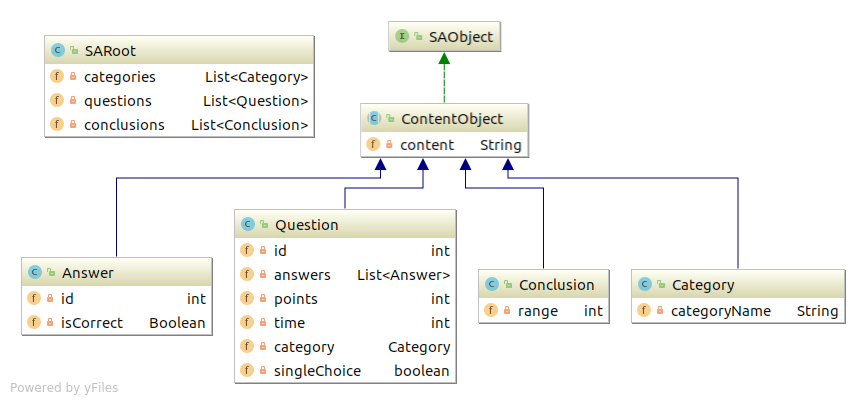
\includegraphics[width = \textwidth]{domain-class-diagram.pdf}
\end{figure*}

Mit Hilfe des Creator GUI, beschrieben in Abschnitt~\ref{Julian}, kann man die Objekte der im Klassendiagramm dargestellten Klassen instanziieren. 
So kann der Ersteller einen Test modellieren.
Aus diesen Objekten kann schließlich direkt eine Webseite generiert werden. 
Die Beschreibung des Generators kann Abschnitt~\ref{Sokol} entnommen werden.

Der Parser, dokumentiert in Abschnitt~\ref{Tim}, bietet die Möglichkeit, die erstellten Objekte in einer XML-Datei zu speichern und sie wieder einzulesen.





\section{Implementierung}

\subsection{Creator}
\section{Julian's Abschnitt}\label{Julian}
\subsection{Hier kommt der erste Teil-Abschnitt }
bliBlaBlub


\subsection{Parser}
\label{Tim}
In diesem Kapitel wird die Parser Komponente vorgestellt. Ihre primäre Aufgabe besteht darin, zwischen dem Speichermedium und dem Generierungsprozess zu vermitteln. Als Speichermedium dienen hierbei einfache XML Dateien, während die aktive Generierung mit Java Objekten arbeitet.\\
Im folgenden wird zunächst die Interne Struktur vorgestellt, welche der Implementierung zugrunde liegt. Anschließend wird die Funktionalitäten der Parser Komponente im Detail vorgestellt. 

\subsection{Interne Struktur}
Generell sind alle hier relevanten Teile eines Self Assessment Tests ( Kategorien, Fragen, Antworten, Ergebnis ) Java Objekte. 
Nachdem eine Frage erstellt wurde ist sie zunächst ein Java Objekt der Klasse 'Question'. Als solches besitzt die Frage verschiedene Attribute wie z.b. ihre Kategorie, den Aufgabentext und insbesondere eine Liste der ihr zugehörigen Antworten. Somit ist gleichzeitig das Mapping zwischen Fragen und Kategorien, sowie zwischen Fragen und Antworten gegeben. Um den ganzen erstellten Test zu sichern genügt es also, eine Liste der Fragen speichern. Der Einfachheit halber haben wir eine Toplevel Klasse namens 'SARoot' eingeführt. Ein Test wird so letztlich durch ein Objekt der Klasse 'SARoot' repräsentiert, welches eine Liste von Fragen und Kategorien, so wie das Ergebnis beinhaltet.   

\subsection{Speichern von Fragen}
Wie in Kapitel 4.2 beschrieben, kann der Ersteller den aktuellen Arbeitsstand speichern, indem er den Test als XML Datei exportiert. In der GUI findet man diese Operation unter 'Export XML'.
Hierbei werden im Hintergrund alle erstellten Java Objekte an die Parser Komponente übergeben, welche diese dann in XML Elemente umwandelt und in einer Datei abspeichert. Genauer gesagt wird hier genau ein Toplevel Objekt übergeben, welches alle Objekte beinhaltet.\\
Intern verwendet die Parser Komponente die 'Java Architecture for XML Binding (JAXB)'\cite{JAXB}. Der von JAXB\cite{JAXB} bereitgestellte 'marshaller' ermöglicht es Java Objekte von spezifizierten Klassen direkt in XML Elemente zu verwandeln und anschließend in eine XML Datei zu schreiben. Um vom 'marshaller' erkannt zu werden benötigen alle unsere Java Klassen die von JAXB\cite{JAXB} vorgeschlagenen XML Tags.\\
Die Parser Komponente nutzt diese Funktion der JAXB\cite{JAXB} API um unser Speichermedium, eine XML Datei, zu erstellen. So können die nur zur Laufzeit existierenden Objekte persistent gespeichert werden.

\subsection{Einlesen von Fragen}
Um gespeicherte Fragen oder ganze Tests wiederverwendbar zu machen, bietet die Parser Komponente die Möglichkeit XML Dateien einzulesen. Es findet als eine Überführung von XML Elementen in Java Objekte statt. Ähnlich wie beim Speichern verwendet die Parser Komponente hierzu wieder eine Funktionalität des JAXB\cite{JAXB} 'marshaller's. Die Funktionalität besteht darin, aus XML Elementen Java Objekte von Klassen mit passenden XML Tags zu erzeugen.\\
Das Resultat des Einlesens ist ein Toplevel Objekt der Klasse 'SARoot'. Aus diesem Objekt kann der gesamte Self Assessment Test erstellt und die Webseite generiert werden. \\
Die GUI greift auf die Parser Komponente zurück um die 'Import XML' Operation durchzuführen. Außerdem ist es dem erfahrenen Ersteller nun möglich den gesamten Self Assessment Test 'von Hand' in einer XML Datei zu verfassen, ohne hierfür die GUI zu verwenden. 






\subsection{Generator}
\label{Sokol}
Für das einfache Verwalten der Webseite, ist es vorgesehen, dass sie statisch ist.
In diesem Fall heißt das, dass es keinen Server geben soll, der dynamisch auf Anfragen des Benutzers reagiert.
Alle dynamischen Funktionen, wie das Laden neuer Fragen, finden auf der Benutzerebene statt.
Der Server liefert dem Benutzer bei Bedarf, also nur statische Dateien.

Der Vorteil dieses Designs ist, dass die Webseitendateien nur ein Mal aus den Java Objekten generiert werden müssen.
Für diese Funktion haben wir uns für die Template Engine Velocity\footnote{\url{http://velocity.apache.org/}} entschieden.

\subsubsection{Velocity}

Velocity erlaubt es Dokumente mit Variablen zu bestücken, die dann von Velocity mit dem Text aus den Java Objekten ersetzt werden.
Diese Dokumente werden Templates genannt.
Dafür werden Velocity das Java Objekt, der Name des Java Objektes in dem Tamplate und das Template an sich übergeben.
Velocity liest daraufhin das Template, sucht sich die Stellen heraus, die Variablen enthalten, und ersetzt diese mit den Inhalten des Java Objektes.

Ein Beispiel eines Velocity Templates ist in Listing~\ref{lst:velocity-example} gegeben.
Für das Beispiel wird angenommen, dass Velocity ein Question Objekt übergeben bekommt.
Dieses Question Objekt hat eine Funktion 'getContent()', die einen String zurückgibt, und eine andere Funktion 'getAnswers()', die eine Liste mit Answer Objekten zurückgibt.
Das Answer Objekt hat wiederum auch eine Funktion 'getContent()'.
Außerdem wird Velocity der Variablenname 'question' und das aufgeführte Template übergeben.

Das Zeichen '\$' in dem Template signalisiert Velocity, dass der danach kommende Text für Velocity vorgesehen ist.
So bemerkt Velocity, dass '\$question', das übergebene Question Objekt referenziert und ruft im ersten Fall die Funktion 'getContent()' auf.
Die Funktion wird ausgewertet und der zurückgegebene String wird an der Stelle des Funktionsaufrufs gesetzt.

Im Beispiel-Template sieht man auch eine 'foreach' Schleife, die mit '\#foreach' beginnt und mit '\#end' endet.
Diese Schleife sorgt dafür, dass der Abschnitt, der sich in der Schleife befindet, so oft geschrieben wird, wie es Answer Objekte in der von 'question.getAnswers()' zurückgegebenen Liste gibt.

Daraufhin wird '\$answer.getContent()' mit der entsprechenden Rückgabe der Answer Objektes ersetzt.


\begin{lstlisting}[basicstyle=\tiny,label={lst:velocity-example},caption={Beispiel eines Velocity Templates.},language=HTML]
<h1>$question.getContent()</h1>
<ul>
#foreach($answer in $question.getAnswers())
<li>$answer.getContent()</li>
#end
</ul>
\end{lstlisting}

\subsubsection{Erstellung der Webseite}
Für alle Dateien der Webseite, die Inhalte von den Java Objekten benötigen, wird eine Template Datei erstellt.
Daraufhin werden die ausgewerteten Templates, mit den anderen für die Webseite benötigten Dateien, in ein ZIP-Archiv gepackt und in einen von dem Benutzer des Generators festgelegten Ort gespeichert.

Um die Webseite dann zu veröffentlichen, müssen die Dateien im Archiv über einen HTTP-Server angeboten werden.





\subsection{Website}
\section{Jena's Abschnitt}\label{Jena}
\subsection{Hier kommt der erste Teil-Abschnitt }
bliBlaBlub


\section{Anwendungsszenario}
\subsection{Programm ausführen}
Zuerst führt man die Datei \textit{TextEditor.java} aus, die wie folgt im Projekt-Ordner zu finden ist:\newline 

\textit{src>>main>>java>>creator>>TextEditor.java}\newline 

Jetzt öffnet sich das Haupt-Fenster des Creators (siehe Abbildung \ref{fig:Bild0}).
\subsection{Fragen hinzufügen}
Nun fügen wir unter File in der Toolbar neue Kategorien mit Fragen und deren Antworten hinzu. Dabei geben wir an, wie viele Punkte eine Antwort gibt, wie viel Zeit sie maximal beötigt, und ob sie Single Choice zulässt an (Abbildung \ref{fig:Bild0}). Nachdem wir angegeben haben welche Anworten korrekt sind, fügen wir noch entsprechende Conclusions hinzu, deren Range angibt, bis zu wie vielen Punkten jene Conclusion am Ende in der Bewertung angezeigt wird. 
\subsection{Webseite generieren}
Falls wir noch nicht fertig sind und eine Pause machen möchten, kann unser Fortschritt als XML-Datei export und zu einem späteren Zeitpunkt wieder importiert werden.\newline Um die letztendliche HTML-Datei zu erstellen clickt man als Nächstes auf \textit{Generate Website} unter \textit{File} und speichert das Projekt mit der inkludierten HTML-Datei in einem beliebigen Ordner.
\subsubsection*{\textit{optional: lokalen Server erstellen}}
Da der Selfassessment-Test einen Server benötigt, kann man, falls man keinen Server besitzt, auch das Ganze auf einem Lokalen Server testen. Dies gelingt zum Beispiel mit \textit{Node.js}.
\subsection{Selfasessment-Test durchführen}
Sobald die Verbindung zu einem Server besteht, kann der Test benutzt werden. Der Test an sich ist sehr intuitiv zu bedienen. Man wählt seine Antworten aus und clickt auf \textit{Next}. Sollte der Timer ablaufen wird die eingeloggte Antwort genommen und zur nächsten Frage gesprungen. Am Ende kann man noch seine Bewertung einsehen.

\section{Zusammenfassung und Ausblick}

\onecolumn
% einfacher Zeilenabstand
\singlespacing
% Literaturliste soll im Inhaltsverzeichnis auftauchen
\newpage
\addcontentsline{toc}{section}{Literaturverzeichnis}
% Literaturverzeichnis anzeigen
\renewcommand\refname{Literaturverzeichnis}

\bibliography{Hauptdatei}
\end{document}